\newpage
\section{Entwicklung}
In diesem Kapitel wird die schrittweise Entwicklung des digitalen Zwillings der robocell beschrieben.
Zunäscht werden alle relevanten Datenquellen identifiziert und geeignete Submodelle der \acs{aas} ausgewählt.
Darauf aufbauend folgt die Modellierung dieser mithilfe des Package Explorers sowie die Validierung mit einer Test Engine.
Im Anschluss wird gezeigt, wie die \acs{aas} mithilfe von Eclipse BaSyx bereitgestelllt und verwaltet werden kann.
Dabei werden sowohl Echtzeidaten über \acs{opcua} als auch Zeitreihendaten über eine InfluxDB eingebunden.
Darüber hinaus wird auf die Entwicklung von drei exemplarischen Anwendungsfällen eingegangen.
Dazu zählt unter anderem der digitale Produktpass, die automatisierte Generierung der \acs{aas} sowie der Einsatz von \acs{ki}.

\subsection{Konzeptionierung des digitalen Zwilling}
Ziel dieses Abschnittes ist es, eine grundlegende Basis für die Erstellung des digitalen Zwillings zu schaffen.
Dabei wird untersucht, welche Daten für die Modellierung erforderlich sind, wo diese herkommen und wie sie in (standardisierten) Submodellen der \acs{aas} strukturiert werden können.
\subsubsection{Identifikation relevanter Datenquellen}
Ein digitaler Zwilling basiert immmer auf einer Vielzahl unterschiedlicher Daten, die gemeinsam ein umfassendes digitales Abbild eines Assets ermöglichen. 
Dabei werden sowohl statische Informationen (z.B. Datenblätter oder Konstruktionsdaten) als auch dynamische Daten, die während des Betriebs einer Maschine anfallen, benötigt.
Im ersten Schritt gilt es daher, alle relevanten Datenquellen zu identifizieren, die für die Modellierung des digitalen Zwillings erforderlich sind.

In industriellen Umgebungen kommen typischerweise verschiedene Systeme zur Erfassung, Verwaltung und Speicherung von Maschinendaten zum Einsatz.
Bei groninger übernimmt diese Funktion das \acs{plm}-System Agile, das eng mit dem \acs{erp}-System PSI Penta verknüpft ist.
Darin sind unter anderem Stücklisten, technische Spezifikationen, \acs{cad}-Dateien sowie allgemeine Dokumente hinterlegt, die die statische Grundlage  für den digitalen Zwilling bilden.

Neben den Informationen aus den Unternehmenssystemen spielen aber auch Laufzeitdaten, wie sie durch Sensoren oder Steuerungssysteme erzeugt werden, eine zentrale Rolle.
Da im Rahmen dieser Arbeit keine reale Maschine angebunden ist, werden diese Daten simuliert.
Hierfür kommt eine in Node.js entwickelte Anwendung zum Einsatz, die im Folgenden als Datengenerator bezeichnet wird und sowohl Prozess- als auch Betriebsdaten generiert. 
Ergänzend dazu wird ein Maschinensimulator verwendet, der einen PackML-Zustandsautomaten abbildet und typische Maschinenzustände sowie deren Übergänge simuliert. 
Beide Komponenten stehen als Docker Container zur Verfügung und stellen die Daten über einen \acs{opcua} Server bereit, wodurch eine realitätsnahe Datenbasis geschaffen wird.
\subsubsection{Auswahl geeigneter Teilmodelle}
Aufbauend auf den zuvor betrachteten Informationsquellen gilt es nun zu entscheiden, welche Aspekte der Maschine im digitalen Zwilling, oder besser gesagt in der \acs{aas}, abgebildet werden sollen.
Im nächsten Schritt ist daher die Auswahl bzw. der Entwurf geeigneter Submodelle erforderlich, die die relevanten Informationen strukturiert bereitstellen.

Als Orientierung dienen die von der \acs{idta} bereitgestellten Submodel Templates \cite{idtaTemplates}, die bereits viele typische Anwendungsfälle standardisiert abdecken.
Diese sind jeweils in einer Submodellspezifikation der \acs{idta} dokumentiert.
Darüber hinaus besteht jedoch auch die Möglichkeit, eigene Submodelle zu entwerfen, die gezielt auf projektspezifische Anforderungen zugeschnitten sind.
Diese können entweder vollständig neu konzipiert oder aus bestehenden Vorlagen abgeleitet werden.

Die konkrete Auswahl der Submodelle in dieser Arbeit orientiert sich hauptsächlich an typischen Industrie 4.0-Anwendungsfällen, die unter anderem auf der Website der \acs{idta} dokumentiert sind \cite{idtaUseCases}.
Diese Anwendungsfälle zeigen auf, welche Submodelle in der Praxis besonders relevant sind.
Eines der wichtigsten ist vermutlich das digitale Typenschild, da dieses häufig die erste Anlaufstelle für die Identifikation und grundlegende Informationen eines Assets darstellt.
Daneben wurden aber auch projektspezifische Anforderungen berücksichtigt, die sich aus den verfügbaren Daten sowie dem fachlichen Austausch mit Industriepartnern wie Wittenstein ergaben.

Tabelle \ref{tab:Submodelle} liefert einen Überblick über die initiale Auswahl dieser Submodelle sowie den zugehörigen Datenquellen.
Diese werden in späteren Anwendungsfällen gezielt erweitert.
Zur besseren Übersicht sind dynamische Submodelle farblich hervorgehoben, während statische Submodelle weiß hinterlegt sind.
Sofern vorhanden, verweist die Spalte Standardisierung auf das jeweils zugehörige Submodel Template mittels der offiziellen Dokumentennummer der \acs{idta}, in der die bettrefende Version spezifiziert ist.
Die in der Spalte Vorgesehene Inhalte genannten Punkte zeigen beispielhaft auf, welche Informationen im weiteren Verlauf im digitalen Zwilling abgebildet werden sollen.

%\newpage
{\small
\begin{longtblr}[
    label = tab:Submodelle,
    entry = Submodelle mit typischen Inhalten,
    caption = {Submodelle mit typischen Inhalten}
  ]{
    colspec = {l l X[c]},
    rowhead = 1,
    vlines,
    hline{1-11} = {-}{},
    }
    \textbf{Submodell}                                   & \textbf{Typische Inhalte}                            & \textbf{Standardisierung} \\
    Typenschild                                          & \makecell[l]{Hersteller \\ Seriennummer \\ Adressinformationen}                  & IDTA 02006-3-0 \cite{SpezifikationTypenschild} \\
    Dokumentation                                     & \makecell[l]{Allgemeine Dokumente \\ Betriebsanleitungen \\ Projektzeichnungen}             & IDTA 02004-1-2 \cite{SpezifikationDokumentation} \\
    3D-Modelle                                           & Konstruktionsmodelle                & IDTA 02026-1-0 \cite{Spezifikation3DModelle}\\*
    Technische Daten                                     & \makecell[l]{Generelle Informationen \\ Technische Eigenschaften }                       & IDTA 02003 \cite{SpezifikaitonTechnischeDaten}\\*
    \acs{bom}                                     &  \makecell[l]{Strukturierte Stücklisten \\ Komponentenbeziehungen }                    & IDTA 02011-1-1 \cite{SpezifikationHierachischeStrukturen}\\*
    Wartung                                              &  \makecell[l]{Wartungsinformationen \\ Wartungsintervalle \\ }          & -  \\*
    Prozessdaten                                         &  \makecell[l]{Messwerte}             & - \\*
    Zeitreihendaten                                       &  \makecell[l]{Zeitreihen }             & IDTA 02008-1-1 \cite{SpezifikationTimeSeriesData}    \\*
    Kontrollkomponente                                   &  \makecell[l]{Betriebsmodi \\ Schnitstelle zur Automatisierung }             & - \\      
\end{longtblr}
}

Im Rahmen dieser Arbeit ist die Modellierung der \acs{aas} bzw. der verschiedenen Submodelle als Instanz vorgesehen.
Auch wenn es sich bei der robocell grundsätzlich um ein generisches Modul innerhalb einer Maschinenfamilie handelt und somit technisch gesehen als Typ klassifiziert werden könnte, steht in diesem Projekt die exemplarische Umsetzung eines konkreten digitalen Zwillings im Vordergrund.
Dies begründet sich vor allem durch die Anbindung von Echtzeit- und Zeitreihendaten sowie die Abbildung einer Betriebsumgebung, was dem digitalen Zwilling einen klaren Instanzcharakter verleiht.
Außerdem unterstützt dies die spätere Demonstration der konkreten \acs{aas} im Industrie 4.0-Systemkontext.
% Im Rahmen dieser Arbeit ist die Modellierung der AAS als Instanz vorgesehen.
% Auch wenn es sich bei der robocell grundsätzlich um ein generisches Modul einer Maschinenfamil technisch um einen Typ handelt und keine
% In diesem Projekt exemplarische Umsertzung eines konkreten digitalen Zwillings im Vordergrund da echtzeitdaten un dzeitreihendaten angebunden werden und eine betriebsumgebung abgtebildet wird instanzcharackter.
% Unterstützt zudem die Demonstration der aasa im Systemkontext.


% Ein besonders wichtiges Submodell stellt die Stückliste (\acs{bom}) dar.
% Mit diesem lässt sich die hierarchische Struktur eines Assets abbilden, das aus mehreren verschachtelten Komponenten besteht.
% Für komplexe Maschinen oder Anlagen, wie im Fall der robocell, wird im Rahmen dieser Konzeption vorgesehen, einzelne ausgewählte Komponenten jeweils als eigene \acs{aas}-Instanzen zu modellieren und in der übergeordneten Haupt-\acs{aas} zu referenzieren.
% Diese werden im weiteren Verlauf als Komponenten-\acs{aas} bezeichnet.
% Auf diese Weise soll eine höhere Modularität und Wiederverwendbarkeit erreicht werden.

% Zur Verdeutlichung der zugrunde liegenden Architektur sowie der Beziehungen zwischen den identifizierten Datenquellen, \acs{aas} und Submodellen dient Abbildung~\ref{fig:konzeptionierungAAS}. 
% Die \acs{aas} der robocell bildet dabei das zentrale digitale Abbild, in das die relevanten Informationen aus den in diesem Kapitel beschriebenen Submodellen integriert werden sollen.

% \begin{figure}[htbp]
%     \centering
%     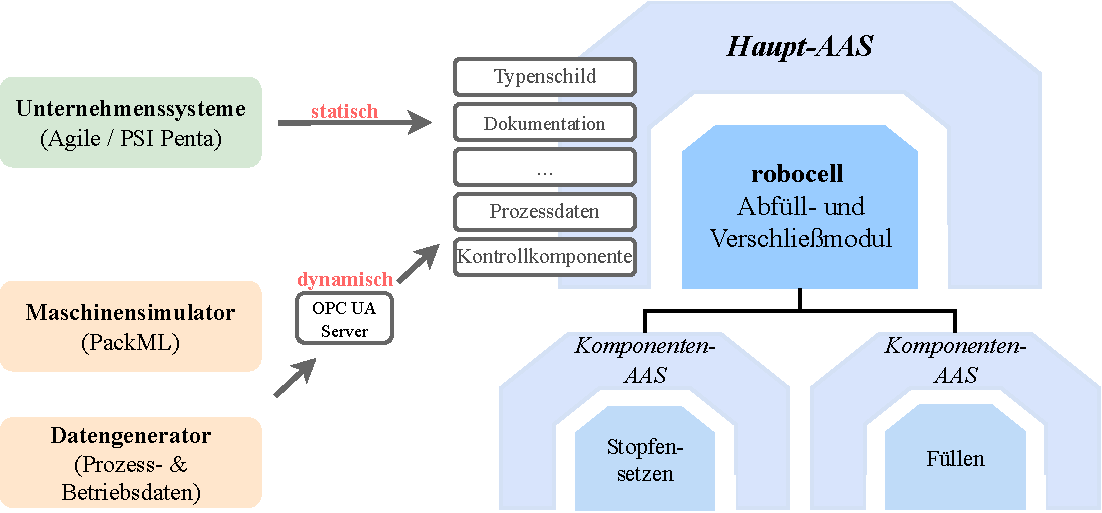
\includegraphics[width=1\textwidth]{Bilder/Konzeptionierung/konzeptionierungNeu.pdf}
%     \caption{\acs{aas}-Konzept der robocell}
%     \label{fig:konzeptionierungAAS}
% \end{figure}

% \medskip
% \noindent
% \textbf{Entitie}\\
% Zur Abbildung hierarchischer Strukturen, insbesondere im Submodell \acs{bom}, werden sogenannte Entities verwendet. 
% Eine Entitie repräsentiert dabei ein untergeordnetes Asset innerhalb der Gesamtstruktur. 
% Grundsätzlich lassen sich zwei Typen unterscheiden. 
% CoManagedEntities besitzen keine eigene \acs{aas} und werden innerhalb der AAS der übergeordneten Hauptkomponente mitverwaltet. 
% SelfManagedEntities hingegen, wie sie im Rahmen der Konzeption dieser Arbeit vorgesehen sind, verfügen über eine eigene \acs{aas} und können somit unabhängig verwaltet und referenziert werden. 
% Die Identifikation erfolgt über die jeweils zugewiesene globalAssetId.

% \medskip
% \noindent
% \textbf{Property}\\
% Das Submodellelement Property dient der Repräsentation einfacher Merkmale eines Assets, wie beispielsweise Name, Seriennummer oder Status. 
% Es ist stets mit einem definierten Datentyp (z. B. string, integer, boolean) verknüpft und lässt sich funktional mit einer Variablen aus der Softwareentwicklung vergleichen.

% \medskip
% \noindent
% \textbf{Property-Element}\\
% Hierbei handelt es sich um ein Datenelement, das einen einfachen Wert (z. B. eine Zahl, einen Text oder ein Datum) speichert und somit Basisinformationen bereitstellt.

% \medskip
% \noindent
% \textbf{File-Element}\\
% Dieses Element dient zum Einbetten oder Verlinken von Dateien, etwa Bildern oder Dokumenten, die dem Asset zugeordnet sind.

% \medskip
% \noindent
% \textbf{Operation-Element}\\
% Es beschreibt eine ausführbare Funktion oder Methode, die auf dem Asset oder Submodell ausgeführt werden kann, und unterstützt so Interaktionen oder Steuerungen.

% \medskip

\newpage
\subsection{Modellierung mit der AAS}
In diesem Abschnitt wird beschrieben, wie die zuvor ausgewählten Submodelle in eine \acs{aas} integriert und mit konkreten Daten sowie semantischen Informationen angereichert werden können.
Dabei wird erläutert, wie eine \acs{aas} von Grund auf modelliert, schrittweise mit Inhalten gefüllt und abschließend gespeichert bzw. exportiert werden kann.  
Die Umsetzung erfolgt mithilfe des Package Explorers, der eine intuitive Modellierung aller relevanten Elemente der \acs{aas} ermöglicht und so den strukturierten Aufbau eines digitalen Zwillings unterstützt.
Außerdem wird gezeigt, wie sich die erstellte \acs{aas} mit einer Test Engine auf eine korrekte und vollständige Struktur überprüfen lässt.

\subsubsection{Praktische Umsetzung mit dem Package Explorer}

Die Modellierung beginnt mit dem Erstellen eines neuen \acs{aas}-Pakets im Package Explorer.
Dieses dient als Container für die digitalen Inhalte eines Assets.  
In der geöffneten Umgebung lässt sich eine neue \acs{aas} anlegen, die sowohl allgemeine als auch assetspezifische Daten enthält. 
Abbildung~\ref{fig:NeuesAASPaket} zeigt den initialen Aufbau im Package Explorer, der im weiteren Verlauf sukzessive um Submodelle und deren Inhalte erweitert wird.
Dateien, wie ein Titelbild für die robocell können dabei bereits zu Beginn in die \acs{aas}-Umgebung eingebettet werden und sind ein integraler Bestandteil des digitalen Zwillings.

\begin{figure}[htbp]
    \centering
    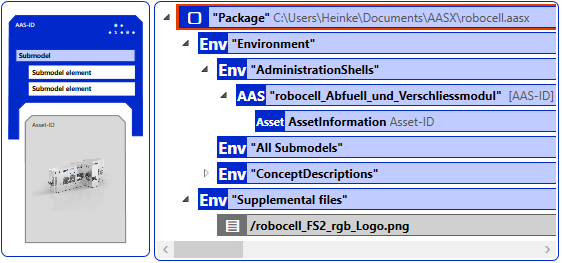
\includegraphics{Bilder/ModellierungAAS/Final/NeuesAASPaket.PNG}
    \caption{AAS-Paket im Package Explorer}
    \label{fig:NeuesAASPaket}
\end{figure}

Anschließend müssen die Metadaten der \acs{aas} sowie des zugehörigen Asset spezifiziert werden.
Neben der Auswahl des Asset-Typs ist insbesondere die eindeutige Identifikation von zentraler Bedeutung.
Das Asset selbst wird über eine globalAssetId referenziert, während die \acs{aas} eine eigene ID und eine idShort erhält.
Diese vereinfachen nicht nur den späteren Austausch der \acs{aas}, sondern ermöglichen auch deren systemweites Auffinden innerhalb eines Industrie-4.0-Ökosystems.
Für erste Modellierungszwecke empfiehlt es sich, auf automatisch generierte Beispiel-IDs zurückzugreifen, die direkt im Package Explorer erzeugt werden können.

\subsubsection*{Strukturierung durch Submodelle}
Im nächsten Schritt müssen die benötigten Submodelle zur \acs{aas} hinzugefügt werden.
Diese lassen sich entweder als Instanz, Typ oder auch Template anlegen, was eine flexible Modellierung je nach Anwendungsfall ermöglicht.
Jedes Submodell erhält dabei wie die \acs{aas} auch eine eindeutige ID, über die diese später identifiziert werden können.
Zusätzlich können optionale Administrationsinformationen angegeben werden, wie beispielsweise die Versionsnummer oder der Name des Autors.

Beim Erstellen eines Submodells ist dieses zunächst leer. 
Die Modellierung erfolgt durch das schrittweise Hinzufügen von Submodellelementen.
Tabelle~\ref{tab:Submodellelemente} gibt einen Überblick über die wichtigsten Submodellelemente, die im Package Explorer zur Verfügung stehen.
Gemäß der Metamodellspezifikation \cite{SpezifikationPart1} wird dabei zwischen DataElements und SubmodelElements unterschieden.
DataElements bilden stets die unterste Ebene im Modell. Sie enthalten konkrete Informationen wie Werte oder Dateien und können keine weiteren Elemente enthalten.
SubmodelElements hingegen sind komplexere Strukturen die wiederum als Container für untergeordnete Elemente dienen.

{\small
\begin{longtblr}[
    label = tab:Submodellelemente,
    entry = Submodellelemente im Package Explorer,
    caption = {Submodellelemente im Package Explorer nach \cite{SpezifikationPart1}},
  ]{
    colspec = {l l X[l]},
    cell{1}{1} = {c=2}{},
    cell{2}{1} = {r=6}{c},
    cell{2}{1} = {bg=babyblue},
    cell{8}{1} = {r=6}{c},
    cell{8}{1} = {bg=babyblue},
    rowhead = 1,
    vline{1,3,4,5} = {-}{},
    vline{2} = {-}{},
    hline{1-2,8,14} = {-}{},
    hline{3-8,9-13} = {2-3}{}, 
    row{1} = {bg=tableHeader},
    }
    \textbf{\makecell[l]{Submodellelement}}& & \textbf{Beschreibung}\\
    \begin{sideways}DataElement\end{sideways}   &Blob & Binärdatei                                                                   \\
    &\makecell[l]{File} & \makecell[l]{Verlinkte oder eingebettete Datei mit \\ eindeutigem MIME-Type}                                                                 \\
    &\makecell[l]{MultiLanguage-\\Property} & Property mit mehrsprachigen Inhalten                              \\
    &Property & Einfaches Merkmal mit festem Datentyp                    \\
    &Range & Wertebereich mit Minimal- und Maximalwert                                                                  \\
    &\makecell[l]{Reference-\\Element} & Verweis auf interne oder externe Elemente                                     \\
    \begin{sideways}SubmodelElement\end{sideways} &Capability & \makecell[l]{Fähigkeit eines Assets, etwas bewirken \\ zu können (ohne konkrete Umsetzung)}                                                            \\
    &Entity & \makecell[l]{Einzelne Komponente (Asset) innerhalb \\ einer übergeordneten AAS  }                                                              \\
    &Operation & \makecell[l]{Funktion mit Ein- und Ausgabeparametern, die \\ von einem System ausgeführt werden kann}                                                               \\
    &\makecell[l]{Relationship-\\Element} & \makecell[l]{Beziehung zwischen zwei Elementen \\(sowohl intern als auch extern möglich)}                                   \\
    &\makecell[l]{Submodel-\\ElementList (\acs{sml})} & \makecell[l]{Geordnete Liste verschiedener Submodellelemente}                                 \\
    &\makecell[l]{SubmodelElement-\\Collection (\acs{smc})} & Sammlung von Submodellelementen                           \\
\end{longtblr}
}

Submodellelemente erhalten im Gegensatz zu Submodellen keine eigene ID, sondern werden über ihre idShort eindeutig referenziert.
Diese muss innerhalb eines Submodells einzigartig sein.
Eine Ausnahme bilden SubmodelElementLists, in denen die enthaltenen Elemente nicht über eine idShort, sondern nur über ihre Position (Index) identifiziert werden.

Ein weiterer wichtiger Punkt sind Referenzen im Package Explorer.
Vlt bekomme ich auch nochmal Entitäten rein


Alternativ zur manuellen Modellierung können die im Rahmen der Konzeption ausgewählten Submodel Templates verwendet werden, wie sie in Tabelle~\ref{tab:Submodelle} aufgeführt sind.
Diese stammen beispielsweise aus dem offiziellen Repository der \acs{idta} \cite{idtaTemplates} und lassen sich als AASX-Dateien importieren.
Im Package Explorer erfolgt dies über ein sogenanntes Auxiliary AAS, das als sekundäre Umgebung zur Template-Verwaltung dient.
Die importierten Templates enthalten eine strukturierte Vorlage mit typischen Submodellelementen und reduzieren somit den Modellierungsaufwand erheblich.
Auch unternehmensspezifische Ableitungen lassen sich darauf aufbauend erstellen.
Ein vertiefter Ansatz zur Template-Nutzung findet sich in Kapitel~\ref{chap:ErstellenvonSubmodelTemplates}.

Nach dem Strukturaufbau können konkrete Inhalte wie Werte, Dokumente oder Referenzen eingepflegt werden.
Dies beschränkt sich jedoch auf statische Submodelle wie Typenschild, Technische Daten oder Dokumentation.
Dynamische Inhalte, etwa Betriebsdaten werden nicht direkt im Package Explorer gepflegt, sondern über externe Datenquellen (z.B. Maschinensimulator oder Datengenerator) angebunden.

\subsubsection*{Semantische Beschreibung mit Concept Descriptions}

Für die semantische Beschreibung von Submodellen und Submodellelementen innerhalb der AAS ist die Vergabe von semanticId-Referenzen essenziell.
Jede semanticId verweist auf eine zugehörige \acs{cd}, die die Bedeutung des referenzierten Elements eindeutig und maschinenlesbar beschreibt.
Im Package Explorer lassen sich solche Concept Descriptions manuell anlegen und verwalten.
Dabei steht eine vordefinierte Eingabemaske zur Verfügung, die sich an dem in Part 3a: Data Specification - IEC 61360 \cite{SpezifikationPart3a} vordefinierten Datenmodell für semantische Beschreibungen orientiert.
Wie in Abbildung \ref{fig:DataSpecificationConten} dargestellt, umfasst diese Vorlage strukturierte Felder wie Definition, Datentyp, Einheit oder Symbol.
Dadurch wird eine konsistente und semantisch eindeutige Beschreibung einzelner Elemente im Submodell ermöglicht.

\begin{figure}[htbp]
    \centering
    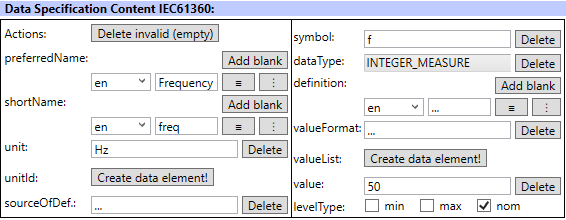
\includegraphics{Bilder/ModellierungAAS/V1/test.png}
    \caption{Package Explorer: Vorlage für Concept Description}
    \label{fig:DataSpecificationConten}
\end{figure}

Alternativ können auch externe Standards referenziert werden. 
Der Package Explorer unterstützt diesen Ansatz durch eine erweiterte Funktionalität, mit der sich vorgefertigte ECLASS-Kataloge direkt in das Tool importieren lassen. 
Nach dem Import können die enthaltenen Objekte durchsucht, ausgewählt und den entsprechenden Submodellen oder Submodellelementen zugewiesen werden. 
Die semantische Verknüpfung erfolgt dabei über eine \acs{irdi}, die das jeweilige Konzept eindeutig identifiziert \cite{eclass_irdi}. 

Wird ein solcher Standard referenziert, legt der Package Explorer automatisch eine \acs{cd} an.
Diese folgt, wie bei der manuellen Erstellung, dem in IEC~61360 definierten Datenmodell.  
So sind die semantischen Informationen auch lokal im Modell verfügbar und konsistent strukturiert.
Technisch betrachtet wäre jedoch auch eine rein externe Referenz ausreichend, da die entsprechenden Elemente bereits vollständig in den jeweiligen Katalogen enthalten sind.
Die Nutzung etablierter externer Standards ist grundsätzlich zu bevorzugen, da sie nicht nur den Modellierungsaufwand erheblich reduziert, sondern auch die Interoperabilität zwischen verschiedenen Systemen und Anwendungen deutlich verbessert.

\subsubsection*{Exportmöglichkeiten im Package Explorer}
Nach Abschluss der Modellierung lässt sich die erstellte \acs{aas} in verschiedenen Formaten exportieren.
Das bevorzugte Format in diesem Projekt ist das AASX-Format, das sich als standardisierte Austauschform für die \acs{aas} etabliert hat.
Es enthält alle modellierten Inhalte, einschließlich eingebetteter Dateien wie Bilder oder Dokumente, und eignet sich daher besonders für die Weitergabe einer Typ-1-\acs{aas}.

Alternativ kann die \acs{aas} auch als JSON- oder XML-Datei gespeichert werden.
Diese Formate beeinhalten allerdings ausschließlich die strukturierte Beschreibung der \acs{aas}, eignen sich jedoch besonders für die Nutzung in APIs oder zur Anbindung an bestehende Softwaresysteme.
Zusätzlich unterstützt der Package Explorer auch den gezielten Export einzelner Submodelle oder Concept Descriptions.
Diese lassen sich seperat, etwa als JSON-Datei abspeichern und können so gezielt in anderen AAS-Projekten wiederverwendet werden.

\subsubsection{Abbildung hierarchischer Strukturen und Beziehungen}
Zur Abbildung hierarchischer Strukturen, insbesondere im Submodell \acs{bom}, werden sogenannte Entities verwendet. 
Eine Entitie repräsentiert dabei ein untergeordnetes Asset innerhalb der Gesamtstruktur. 
Grundsätzlich lassen sich zwei Typen unterscheiden. 
CoManagedEntities besitzen keine eigene \acs{aas} und werden innerhalb der AAS der übergeordneten Hauptkomponente mitverwaltet. 
SelfManagedEntities hingegen, wie sie im Rahmen der Konzeption dieser Arbeit vorgesehen sind, verfügen über eine eigene \acs{aas} und können somit unabhängig verwaltet und referenziert werden. 
Die Identifikation erfolgt über die jeweils zugewiesene globalAssetId.

\subsubsection{Validierung}
Im Anschluss an die Modellierung der \acs{aas} sollte eine Überprüfung der Konformität erfolgen.
Hierzu kann eine von der \acs{idta} bereitgestellte Test Engine \cite{TestEngine} eingesetzt werden. 
Diese lässt sich direkt mit pip, dem Paktemanager von Python, installieren und anschließend über die Kommandozeile nutzen.
Mit dem Befehl \verb|aas_test_engines check_files robocell.aasx| kann beispielsweise die Validierung der zuvor erstellten AASX-Datei der robocell gestartet werden.

Dabei wird zunächst geprüft, ob die AASX-Datei formal korrekt aufgebaut ist, insbesondere hinsichtlich der internen Struktur und ihrer Beziehungen.
Anschließend erfolgt die Kontrolle der enthaltenen \acs{aas} gegen die Metamodell-Spezifikationen der \acs{idta} (Teil 1 \cite{SpezifikationPart1} und 3a \cite{SpezifikationPart3a}).
Zuletzt erfolgt ein Abgleich der Submodelle mit den zugehörigen Templates, sofern diese für das jeweilige Submodell definiert wurden.

Treten bei der Validierung formale oder semantische Fehler auf, beispielsweise durch fehlende Referenzen oder ungültige IDs, gibt die Test Engine eine detaillierte Fehlermeldung in der Konsole aus. 
Diese Hinweise geben Aufschluss darüber, an welcher Stelle die Struktur bzw. der Inhalt der AASX-Datei fehlerhaft ist, und ermöglichen so eine gezielte Korrektur der betroffenen Elemente. 
Werden im gesamten Prüfprozess hingegen keine Fehler oder Abweichungen festgestellt, bestätigt die Test Engine die erfolgreiche Validierung.

\newpage
\subsection{Technische Integration}
Im Anschluss an die Konzeption und Modellierung des digitalen Zwillings liegt der Fokus dieses Kapitels auf der technischen Integration der zuvor erstellten \acs{aas} in eine Industrie-4.0-kompatible Umgebung.
Dabei wird unter anderem gezeigt, wie die statisch modellierte Typ-1-\acs{aas} mithilfe des AASX Server Blazor beziehungsweise vorzugsweise der Eclipse BaSyx-Plattform in eine Typ-2-\acs{aas} überführt und systemseitig bereitgestellt werden kann.
Ergänzend dazu wird beschrieben, wie die \acs{aas} um dynamische Inhalte erweitert werden kann.
Dies umfasst die Integration von Echtzeitdaten über OPC UA sowie die Einbindung und Visualisierung externer Zeitreihendaten mithilfe von InfluxDB und Telegraf.

\subsubsection{Bereitstellung der \acs{aas}}
\label{sec:bereitstellungAAS}
Für die Bereitstellung als Typ-2-\acs{aas} stehen verschiedene Open-Source-Lösungen zur Verfügung. 
Eine besonders einsteigerfreundliche Option stellt der AASX Server Blazor \cite{AASXServer} dar.
Er bildet das serverseitige Gegenstück zum Package Explorer und verfügt ebenfalls über eine grafische Benutzeroberfläche zur Visualisierung von \acs{aas}-Paketen.
Über eine HTTP-Schnittstelle können die beiden Anwendungen miteinander verbunden werden.
Dadurch lassen sich AASX-Dateien ohne zusätzlichen Konfigurationsaufwand direkt aus dem Package Explorer heraus auf den Server übertragen und bereitstellen.
Ebenso können auf dem Server gespeicherte \acs{aas} über den Explorer eingesehen und bearbeitet werden.
Die enge Verzahnung beider Komponenten ermöglicht somit eine unkomplizierte Bereitstellung und Verwaltung von \acs{aas}-Paketen und eignet sich besonders für erste Testszenarien oder prototypische Anwendungen.

Für komplexere Anwendungsszenarien, insbesondere solche mit Anforderungen an Echtzeitfähigkeit sowie an flexible und erweiterbare Submodelle, stößt der AASX Server Blazor jedoch an seine funktionalen und architektonischen Grenzen. 
So fehlen beispielsweise Schnittstellen zur Anbindung dynamischer Datenquellen sowie Möglichkeiten zur Skalierung und zur verteilten Systemintegration.
Aus diesem Grund wird im weiteren Verlauf dieses Projekts die Eclipse BaSyx-Plattform eingesetzt.
Durch ihre modulare Architektur und die klare Trennung verschiedener Komponenten wie den Registries oder den Repositories bietet sie eine deutlich flexiblere Grundlage für die Umsetzung anspruchsvoller Industrie 4.0-Szenarien.

Die einfachste Möglichkeit, BaSyx zu installieren, besteht in der Nutzung von Docker.
Alle benötigten Komponenten stehen als vorgefertigte Images öffentlich über den Docker Hub zur Verfügung. 
Alternativ kann der Quellcode von GitHub bezogen werden, um einzelne Komponenten individuell anzupassen oder zu erweitern.
Die verschiedenen Services, darunter die \acs{aas} Environment, Registries für \acs{aas} und Submodelle, der Discovery Service, sowie die MongoDB als persistenter Speicher, können zentral in einer docker-compose.yml-Datei verwaltet werden.
Die Konfiguration erfolgt in der Regel über Umgebungsvariablen oder seperate Konfigurationsdateien, die in der docker-compose.yml referenziert werden.
Mit dem Befehl docker compose up lassen sich anschließend alle Komponenten gemeinsam starten.

Nach erfolgreichem Start der BaSyx-Umgebung stehen verschiedene Möglichkeiten zur Verfügung, um eine \acs{aas} bereitzustellen und in das System zu integrieren. 
Welche Methode dabei zum Einsatz kommt, hängt stark von den jeweiligen Anforderungen und Rahmenbedingungen des Anwendungsszenarios ab.
Nachfolgend werden drei ausgewählte Ansätze zur Bereitstellung näher betrachtet.


\paragraph*{a) Volume}
Eine besonders einfache Variante besteht darin, eine AASX-Datei in ein gemountetes Volume der AAS Environment abzulegen.
Ein Volume ist ein persistentes Speicherverzeichnis auf dem Host-System, das mit einem Verzeichnis innerhalb eines Docker-Containers verknüpft ist.
Es ermöglicht die dauerhafte Speicherung von Daten, unabhängig vom Lebenszyklus des Containers.
In der von Eclipse BaSyx bereitgestellten Docker-Umgebung ist ein entsprechendes Volume in der Regel bereits vorkonfiguriert.

Beim Neustart der AAS Environment wird die AASX-Datei automatisch erkannt, registriert und in das BaSyx-System eingebunden.
Die dabei erzeugten Daten, darunter Informationen zu \acs{aas}, Submodellen, Concept Descriptions sowie Registrierungsdaten, werden in verschiedenen Tabellen der angebunden MongoDB gespeichert.
Dies gewährleistet, dass alle relevanten Daten persistent erhalten bleiben, selbst dann, wenn die ursprüngliche AASX-Datei später aus dem Volume entfernt wird.

\paragraph*{b) AAS Web UI}
Alternativ kann die Bereitstellung auch direkt über die AAS Web UI erfolgen.
Über die Benutzeroberfläche kann eine AASX-Datei manuell importiert werden, wodurch sie direkt im laufenden System registriert und eingebunden wird.
Diese Methode eignet sich besonders gut für Tests oder kleinere Anpassungen, da eine \acs{aas} auf diese Weise schnell und ohne direkten Zugriff auf das zugrunde liegende Dateisystem eingebunden werden kann.

\paragraph*{c) REST-API}
Die flexibelste, jedoch auch technisch anspruchsvollste Methode zur Bereitstellung einer AAS ist die manuelle Registrierung über die REST-API. 
Dabei kann nicht einfach eine AASX-Datei hochgeladen werden. 
Stattdessen müssen die AAS, ihre Submodelle sowie deren Beziehungen explizit über die bereitgestellten Schnittstellen des BaSyx-Systems erstellt werden. 
Dies erfolgt durch das Senden strukturierter JSON-Daten im Body der jeweiligen HTTP-Anfragen.
Ein typischer Ablauf dieser Registrierung ist in Tabelle \ref{tab:BereitstellungInBaSyx} dargestellt. 
Sie zeigt die notwendigen Schritte sowie die zugehörigen REST-Endpunkte.
Diese sind dabei verschiedenen Services innerhalb der AAS Environment zugeordnet.

{\small
\begin{longtblr}[
  label = tab:BereitstellungInBaSyx,
  caption = {Bereitstellung einer AAS über die REST-API},
  entry = Bereitstellung einer AAS über die REST-API
]{
  colspec = {l l X},
  rowhead = 1,
  vlines,
  hlines,
  row{1} = {bg=tableHeader}
}
\textbf{Schritt} & \textbf{Service} & \textbf{Endpunkte} \\
1. AAS erstellen & AAS Repository & \texttt{/shells}\\
2. Submodell(e) erstellen & Submodel Repository & \texttt{/submodels}\\
\makecell[l]{3. Submodell(e) mit \\ \acs{aas} verknüpfen} & AAS Repository & \texttt{\makecell[l]{/shells/{\{aasIdentifier\}} \\ /submodel-refs}}\\
4. \acs{cd} anlegen & \acs{cd} Repository & \texttt{/concept-descriptions}\\
\end{longtblr}
}

Neben der Bereitstellung in der AAS Environment kann eine \acs{aas} optional auch im Discovery Service registriert werden.
Über einen sogenannten assetLink kann diese dabei logisch mit ihrem zugehörigen Asset verknüpft werden.
Die Registrierung erfolgt analog zur AAS Environment über einen REST-Endpunkt.
Besonders bei der Darstellung von hierarchischen Strukturen, etwa einer \acs{bom} mit mehreren verschachtelten Assets, hilft der Discovery Service bei der eindeutigen Zuordnung der jeweiligen \acs{aas} zu ihrem physischen Gegenstück.

\subsubsection{Integration von Echtzeitdaten über OPC UA}
Nach der Erstellung der statischen \acs{aas} der robocell und der Integration in das BaSyx-System gilt es nun, diese um dynamische Informationen zu erweitern.
Diese sind essenziell, um den aktuellen Maschinenzustand präzise und in Echtzeit abzubilden.
Die Datenbasis bilden die beiden zuvor vorgestellten Anwendungen, die Maschinen- bzw. Sensordaten über einen \acs{opcua} Server bereitstellen.

Die Integration von Echtzeidaten in die \acs{aas} wird im Folgenden am Beispiel des Submodells Prozessdaten erläutert.
Innerhalb dieses Submodells existieren verschiedene Properties, die jeweils bestimmte Werte, wie beispielsweise den Druck oder die Anzahl abefüllter Einheiten, repräsentieren (siehe Abbildung \ref{fig:SubmodellProzessdaten}). %(siehe Abbildung \ref{fig:UMLSubmodellProcessData}). 
Diese Properties sollen im weiteren Verlauf dynamisch mit den simulierten Werten, die über \acs{opcua} bereitgestellt werden, aktualisiert werden.

\begin{figure}[htbp]
    \centering
    % 0.88
    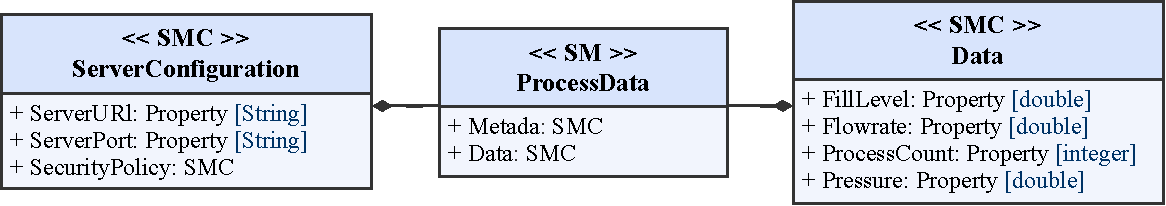
\includegraphics{Bilder/OPCUA/SubmodellProzessdaten.pdf}
    \caption{Submodell Prozessdaten}
    \label{fig:SubmodellProzessdaten}
\end{figure}

Das Eclipse BaSyx-Projekt stellt hierfür eine weitere Komponente bereit, die sogenannte Databridge \cite{BaSyxDatabridge}.
Diese steht, wie alle anderen Komponenten auch, als Docker Container zur Verfügung und ermöglicht die Anbindung verschiedenster Datenquellen an eine \acs{aas}.
Sie unterstützt eine Vielzahl von Protokollen, darunter insbesondere auch \acs{opcua} oder MQTT.
Dabei dient sie als Vermittler zwischen einem Datenendpunkt und einem Submodell innerhalb der \acs{aas}.

Die Konfiguration der Databridge erfolgt über mehrere JSON-Dateien.
In einer zentralen Konfigurationsdatei werden sowohl die Datenquelle als auch die Datensenke definiert.
Außerdem können Transformatoren angegeben werden, die beispielsweise Einheitenumrechnungen oder Typkonvertierungen übernehmen.

Als Datenquelle muss der \acs{opcua} Server des Datengenerators angegeben werden, dessen Konfiguration typischerweise in einer separaten JSON-Datei erfolgt.
Darin sind sowohl die Verbindungsparameter des Servers (z.B. URL und Port) als auch die zu überwachenden Knoten anzugeben.
Wie in Abbildung \ref{fig:OPCUADatenStruktur} zu erkennen, stellt der \acs{opcua} Server die Werte hierfür in einer hierarchischen Struktur bereit, wobei jeder Knoten über einen Namespaceindex (ns) und eine NodeId (i) eindeutig adressierbar ist.

\begin{figure}[htbp]
    \centering
    % 0.88
    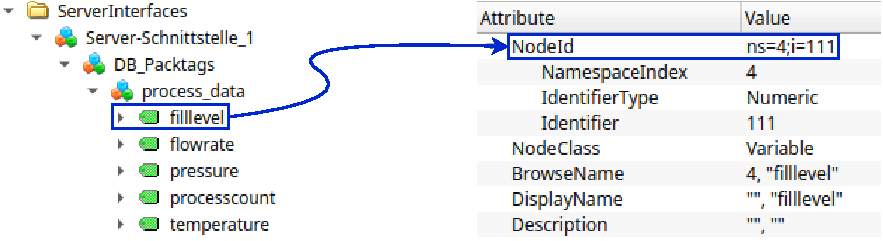
\includegraphics{Bilder/OPCUA/OPCUADaten.pdf}
    \caption{OPC UA Datenknoten}
    \label{fig:OPCUADatenStruktur}
\end{figure}

Außerdem muss der zu verwendende \acs{opcua} Client festgelegt werden.
In diesem Projekt wird Eclipse Milo eingesetzt, der auf einem Subscription-Modell basiert.
Im Gegensatz zu einem Polling-Ansatz werden hier gezielt bestimmte Knoten (Nodes) abonniert, sodass neue Werte automatisch bei Änderung übermittelt werden.

Ein Beispiel für eine entsprechende JSON-Konfiguration der Datenquelle ist in Listing~\ref{lst:jsonDatenquelle} für den Druckwert dargestellt.
Weitere optionale Parameter, wie etwa Sicherheitseinstellungen oder das Übertragungsintervall können zusätzlich angegeben werden, wurden hier jedoch zur besseren Übersicht weggelassen.

\begin{lstlisting}[language=json, caption={Beispielhafte JSON-Konfiguration einer Datenquelle}, label={lst:jsonDatenquelle}]
{
    "uniqueId"       : "pressure",
    "nodeInformation": "ns=4;i=113",
    "serverUrl"      : "opcua-server",
    "serverPort"     : 4840,
    "pathToService"  : "milo"
}
\end{lstlisting}

Zur Anpassung der eingehenden Daten an die Struktur der Ziel-Property lassen sich verschiedene Transformatoren einsetzen.
Die Databridge unterstützt hierfür unter anderem JSONata-Ausdrücke oder JsonJacksonTransformers.
Mithilfe dieser Mechanismen können die vom \acs{opcua}-Server empfangenen Rohdaten zunächst in ein JSON-Objekt überführt und anschließend gezielt extrahiert und weiterverarbeitet werden.

Im Anschluss erfolgt die Konfiguration der Datensenke, also der Zielkomponente innerhalb der \acs{aas}.
Auch diese Konfiguration erfolgt über eine separate JSON-Datei, in der der Endpunkt des Submodells, der idShortPath der gewünschten Property sowie die verwendete API-Version definiert werden.
Listing~\ref{lst:jsonDatensenke} zeigt ein Beispiel einer entsprechenden Konfiguration.
Der Platzhalter \{smId\} steht dabei für die Base64-kodierte ID des Submodells Prozessdaten, wie sie in der REST-API der \acs{aas} verwendet wird.
\begin{lstlisting}[language=json, caption={Beispielhafte JSON-Konfiguration einer Datensenke}, label={lst:jsonDatensenke}]
{
    "uniqueId"        : "Submodel/ProcessData/Pressure",
    "submodelEndpoint": "http://aas-env:8081/submodels/{smId}",
    "idShortPath"     : "Pressure",
    "api"             : "DotAAS-V3"
}
\end{lstlisting}

Nach erfolgreicher Konfiguration übernimmt die Databridge die automatisierte Übertragung der \acs{opcua}-Werte in die entsprechenden Properties des Submodells.
Dieses Prinzip lässt sich nicht nur auf Prozesswerte anwenden, sondern auch zur Abbildung des Maschinenzustands oder anderer dynamischer Betriebsdaten nutzen.
Somit bildet die Databridge eine flexible und protokolloffene Lösung zur Echtzeitanbindung externer Datenquellen an eine \acs{aas}.


\subsubsection{Verarbeitung von Zeitreihendaten}

Grundsätzlich lassen sich Zeitreihendaten auf unterschiedlichste Weise in eine \acs{aas} einbinden.
Das Submodel Template Time Series Data \cite{SpezifikationTimeSeriesData} bietet hierfür mehrere standardisierte Lösungsansätze.
Eine Möglichkeit besteht darin, diese direkt über ein InternalSegment in der \acs{aas} zu speichern.
Diese Variante eignet sich jedoch nur für kleinere Datenmengen.
Alternativ können die Daten in Form einer Datei abgespeichert werden.
Diese können dann entweder direkt in die \acs{aas} eingebunden oder extern über ein ExternalSegment referenziert werden.
Für größere Datenmengen bietet sich die exterene Speicherung an einem seperaten Ort, wie etwa einer Datenbank, an.
Diese kann über ein LinkedSegment mit der \acs{aas} verknüpft werden.

Im Folgenden wird die zuletzt genannte Option näher betrachtet.
Hierzu werden die simulierten Werte für Druck und Temperatur des Datengenerators extern in einer InfluxDB gespeichert.
Die über \acs{opcua} bereitgestellten Daten werden dabei mithilfe von Telegraf, einem leichtgewichtigen Agenten zur Datenerfassung und -weiterleitung \cite{Influx}, kontinuierlich in eine speziell für diesen Anwendungsfall angelegte Tabelle geschrieben.
InfluxDB sowie Telegraf stehen dabei beide als Docker-Container zur Verfügung und lassen sich so nahtlos in das bestehende BaSyx-System integrieren.

Um die in der Datenbank gespeicherten Daten in die \acs{aas} einzubinden, kann das bereits genannte Submodel Template Time Series Data verwendet werden.
Zunächst müssen die Metadaten eingetragen werden (siehe Abbildung \ref{fig:MetadataTimeSeries}).
Dazu gehören ein eindeutiger Name, eine Beschreibung sowie die Definition der Datenpunkte (Records), die hiermit aufgezeichnet werden sollen.

\begin{figure}[htbp]
    \centering
    % 0.88
    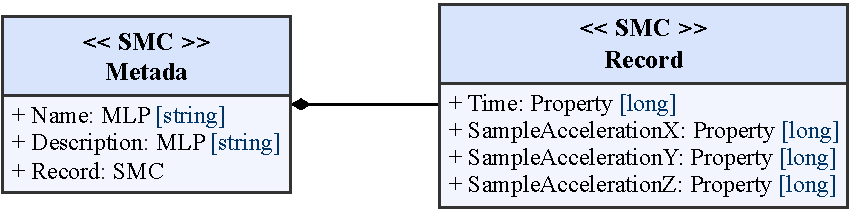
\includegraphics[width=1\textwidth]{Bilder/TimeSeries/Metadaten.pdf}
    \caption{Metadaten im Submodell Time Series Data}
    \label{fig:MetadataTimeSeries}
\end{figure}

Anschließend folgt die Konfiguration des LinkedSegments (siehe Abbildung \ref{fig:LinkedSegmentTimeSeries}). 
Dieses stellt die eigentliche Verbindung zu den extern gespeicherten Zeitreihendaten her.
Hierfür sind sowohl der Datenendpunkt als als auch die Query, mit der die gewünschten Werte ausgelesen werden sollen, zu spezifizieren.
Im vorliegenden Fall handelt es sich dabei um die Adresse des InfluxDB-Containers sowie die Abfrage, mit der die Werte für Druck und Temperatur aus der zugehörigen Tabelle extrahiert werden können.
Dabei ist zu beachten, dass der entsprechende Port der InfluxDB nach außen freigegeben ist, da andernfalls kein Zugriff durch externe Anwendungen möglich ist.
Ergänzend können weitere Metadaten angegeben werden, beispielsweise die Abtastrate (samplingRate), der durch das Segment abgedeckte Zeitraum oder ein recordCount, der die erwartete Anzahl an Einträgen innerhalb dieses Zeitfensters beschreibt.

\begin{figure}[htbp]
    \centering
    % 0.86
    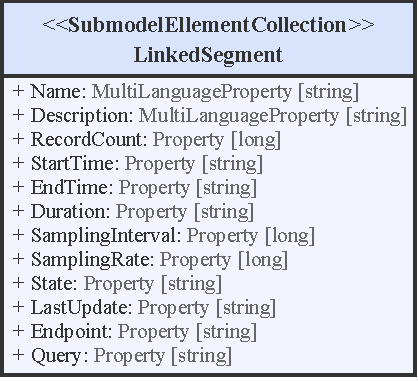
\includegraphics{Bilder/TimeSeries/LinkedSegment.pdf}
    \caption{LinkedSegment im Submodell Time Series Data}
    \label{fig:LinkedSegmentTimeSeries}
\end{figure}

Zur Visualisierung der Zeitreihendaten bietet das BaSyx-System eine praktische Lösung.
Über ein entsprechendes Plugin können die im Submodell Time Series Data enthaltenen Informationen direkt in der Benutzeroberfläche der AAS Web UI dargestellt werden.
Die über das LinkedSegment referenzierten Zeitreihendaten lassen sich dort in verschiedenen Diagrammen visualisieren, beispielsweise als Linien- oder Balkendiagramm.
Dadurch wird eine benutzerfreundliche Darstellung der Daten ermöglicht, ohne dass diese physisch in der \acs{aas} gespeichert werden müssen.

\newpage
\subsection{Anwendungsfall Digitaler Produktpass}
Im Kontext steigender Anforderungen an Nachhaltigkeit und Transparenz enlang des gesamten Produktlebenszyklus eines Assets gewinnt der \acs{dpp} zunehmend an Bedeutung.
Im Folgenden wird daher gezeigt, wie dieser mithilfe der \acs{aas} umgesetzt werden kann. 

Der Anwendungsfall orientiert sich dabei an dem von der ZVEI vorgestellten \acs{dpp40}, dessen beispielhafte Umsetzung unter anderem im Rahmen eines von ZVEI und \acs{idta} entwickelten \acs{pcf}-Showcases \cite{PCFShowcas} demonstriert wird. 
Der Fokus liegt unter anderem auf der Bereitstellung nachhaltigkeitsbezogener Informationen sowie der Umsetzung der im \acs{dpp} geforderten Zugriffsrechte für unterschiedliche Interessensgruppen.
Diese Aspekte sollen im nachfolgenden Abschnitt technisch umgesetzt werden.

Als Grundlage dient der digitale Zwilling der robocell, der im Rahmen dieses Anwendungsfalls um ein Submodell zur Abbildung des Carbon Footprints erweitert wird.
Die Umsetzung der Zugriffsrechte erfolgt mit der Eclipse BaSyx-Plattform, mit der eine rollenbasierte Zugriffskontrolle implementiert werden kann.

\subsubsection{Umsetzung mit dem Teilmodell Carbon Footprint}
Der \acs{pcf} beschreibt die Summe aller Treibhausgasemissionen, ausgedrückt in CO\textsubscript{2}-Äquivalenten, die entlang des Lebenszyklus eines Produkts entstehen \cite{PCF}. 
Zur strukturierten Erfassung dieser Werte kann das von der \acs{idta} spezifizierte Submodel Template Carbon Footprint \cite{SpezifikaitonPCF} eingesetzt werden.

Im Rahmen dieses Anwendungsfalls werden die Phasen Produktion, Material sowie die Gesamtbetrachtung (Cradle to Gate) berücksichtigt. 
Für jede Phase wird gemäß der Submodellspezifikation eine SubmodelElementCollection angelegt, die zentrale Informationen wie den CO\textsubscript{2}-Wert, die Berechnungsmethode sowie den Gültigkeitszeitraum enthält. 
Diese Sammlungen dienen als Grundlage für die spätere Aggregation der \acs{pcf}-Werte der Gesamtmaschine und werden im weiteren Verlauf dynamisch mit Werten befüllt.

Zur Ermittlung dieser Werte wird das Submodell um eine Komponentenliste erweitert, die auf die in der robocell verbauten Steuerungskomponenten verweist. 
Diese Liste bildet die Grundlage für die spätere Berechnung. 
Im Rahmen dieser Arbeit wurde exemplarisch eine Auswahl an Siemens-Komponenten betrachtet, darunter beispielsweise eine CPU sowie Ein- und Ausgangsmodule. 
Diese wurden als Typ-1-\acs{aas} zur Verfügung gestellt, wobei jede \acs{aas} ein eigenes Carbon Footprint-Submodell enthält.

Sowohl die aktualisierte \acs{aas} der robocell als auch die zugehörigen Komponenten-\acs{aas} können über die Eclipse BaSyx-Plattform bereitgestellt werden. 
Die Inhalte lassen sich so direkt über die Benutzeroberfläche der AAS Web UI einsehen. 
Zusätzlich steht ein Plugin zur Verfügung, das die Visualisierung der \acs{pcf}-Werte unterstützt.

Die dynamische Aggregation des \acs{pcf} der Gesamtmaschine erfolgt über eine externe Node.js-API, die über eine im Vue.js-basierten Plugin integrierte Schaltfläche ausgelöst wird. 
Alternativ wäre auch eine direkte Berechnung im Plugin oder über einen Microservice denkbar. 
In der vorliegenden Umsetzung liegt die gesamte Aggregationslogik jedoch serverseitig in der API.
Zur Veranschaulichung ist der Ablauf der Aggregation in Abbildung \ref{fig:SequenzdiagrammPCF}  als Sequenzdiagramm dargestellt.

\begin{figure}[htbp]
    \centering
        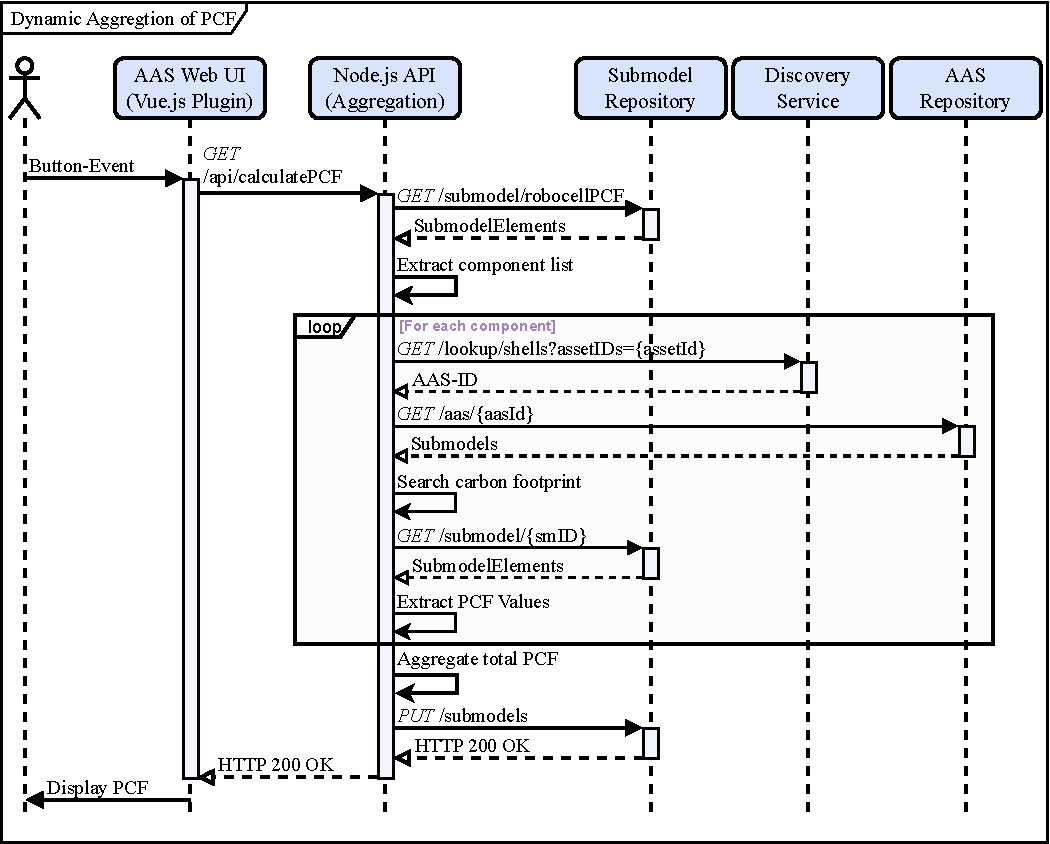
\includegraphics[width=1\textwidth]{Bilder/DPP/Sequenzdiagramm.pdf}
    
    \caption{Sequenzdiagramm zur Aggregation des PCF}
    \label{fig:SequenzdiagrammPCF}
\end{figure}

Die API nutzt dabei die REST-Schnittstelle des Submodel Repositories der AAS Environment, um zunächst alle in der \acs{aas} der robocell hinterlegten Komponenten auszulesen. 
Diese sind jeweils über ihre globalAssetId eindeutig referenziert. 
Mithilfe des Discovery Services werden auf Basis dieser IDs die zugehörigen Komponenten-AAS identifiziert und anschließend vom AAS Repository abgerufen. 
Für jede dieser Komponenten wird geprüft, ob ein Carbon Footprint-Submodell vorhanden ist. 
Falls dies zutrifft, wird das Submodell ausgelesen und die enthaltenen Werte extrahiert.

Aus den ermittelten Einzelwerten berechnet die API schließlich die aggregierten CO\textsubscript{2}-Äquivalente für die Phasen Produktion, Material sowie Cradle to Gate. 
Die berechneten Werte werden abschließend in das Carbon Footprint-Submodell der Haupt-\acs{aas} der robocell geschrieben und stehen dort strukturiert zur Verfügung.

Die beschriebene Lösung ermöglicht es, den \acs{pcf} dynamisch auf Basis der in der Komponentenliste referenzierten Steuerungselemente zu berechnen. 
Auch wenn derzeit nur ausgewählte Komponenten berücksichtigt werden, lässt sich die Liste bei Verfügbarkeit weiterer Komponenten-\acs{aas} unkompliziert erweitern, sodass sukzessive die gesamte Maschine in die Berechnung einbezogen werden kann. 
Perspektivisch lässt sich die Berechnung zudem um weitere Lebenszyklusphasen wie Nutzung oder Entsorgung ergänzen, um eine ganzheitliche Betrachtung von der Herstellung bis zum Lebensende eines Produkts bzw. einer Maschine zu ermöglichen.

\subsubsection{Zugriffsrechte und Datensicherheit}
Das vlt zu komplex \dots
Einfach weglassen ? 


\newpage
\subsection{Anwendungsfall automatisierte Generierung von AAS}
Ziel dieses Anwendungsfalles ist es, den Prozess der automatisierten Generierung und Bereitstellung einer \acs{aas} darzustellen.
Dazu wird zunächst ein Submodel Template im Package Explorer erstellt und anschließend in ein Typ-Submodell überführt.
Dieses wird anschließend automatisiert mit Daten befüllt, in eine \acs{aas}-Instanz eingebettet und schließlich in ein Industrie 4.0-System eingebunden.

\subsubsection{Erstellen von Submodel Templates}
\label{chap:ErstellenvonSubmodelTemplates}
Das Erstellen von Submodel Templates spielt eine zentrale Rolle für den effizienten Einsatz der \acs{aas} in Industrie 4.0-Anwendungen. 
Ein einmal definiertes Template kann für beliebig viele Instanzen eines digitalen Zwillings wiederverwendet werden. 
Dadurch wird nicht nur die Konsistenz der Datenstruktur sichergestellt, sondern auch der Entwicklungsaufwand erheblich reduziert.

Grundsätzlich gibt es mehrere Möglichkeiten ein solches Template zu erstellen.
Es kann entweder vollständig neu modelliert oder von bestehenden Submodel Templates abgeleitet werden, wie es im Folgenden exemplarisch anhand des Submodells Technische Daten \cite{SpezifikaitonTechnischeDaten} gezeigt wird.
Dieses Template stellt eine standardisierte Struktur zur Beschreibung technischer Merkmale eines Produkts bereit.

Für die technische Umsetzung kann der Package Explorer eingesetzt werden.
Hierfür muss zunächst das Submodel Template Technische Daten importiert werden.
Dabei handelt es sich um ein generisches Template, das lediglich grundlegende Strukturkategorien vorgibt.
Es enthält beispielsweise SubmodelElementCollections wie Generelle Informationen, Technische Informationen oder Produktklassifikation, die allerdings noch nicht mit konkreten Eigenschaften gefüllt sind.

Auf Unternehmensebene kann dieses Template für eine bestimmte Produktgruppe mit zusätzlichen Merkmalen individualisiert werden.
So lassen sich beispielsweise spezifische Anforderungen bzw. produktspezifische Eigenschaften wie Umgebungsbedingungen oder elektrische Daten einer Maschine ergänzen.

Aus dem angepassten Template kann anschließend eine Typ-\acs{aas} erstellt werden, in die bereits konkrete allgemeingültige Merkmale einer Produktgruppe eingetragen werden.
Diese dient als Vorlage für die spätere Instanziierung konkreter digitaler Zwillinge einzelner Produkte, bei denen dann auch die produktspezifischen Werte ergänzt werden.
Zur Weiterverwendung kann das Submodell direkt im Package Explorer als JSON-Datei exportiert werden.
% Das Erstellen von Submodel Templates spielt eine wichtige Roll für den späteren Einsatz\dots
% Einmal ein Submodel template erstelllen, später für alle Insatnzen wiederverwendet werden
% Dies spart enorm an Zeit bei der Entwicklung 

% Eine Möglichkeit zur Erstellung der Templates mit dem Package Explorer
% Hierfür kann er als Expertentool eingesetzt werden
% Dort kann das strukturiert aufgebaut werden
% Das ist dann ein Template und kann anschließend mit Daten gefüllt werden.


% Beispiel technische Daten mit Abbildung

% \begin{figure}[htbp]
%     \centering
%     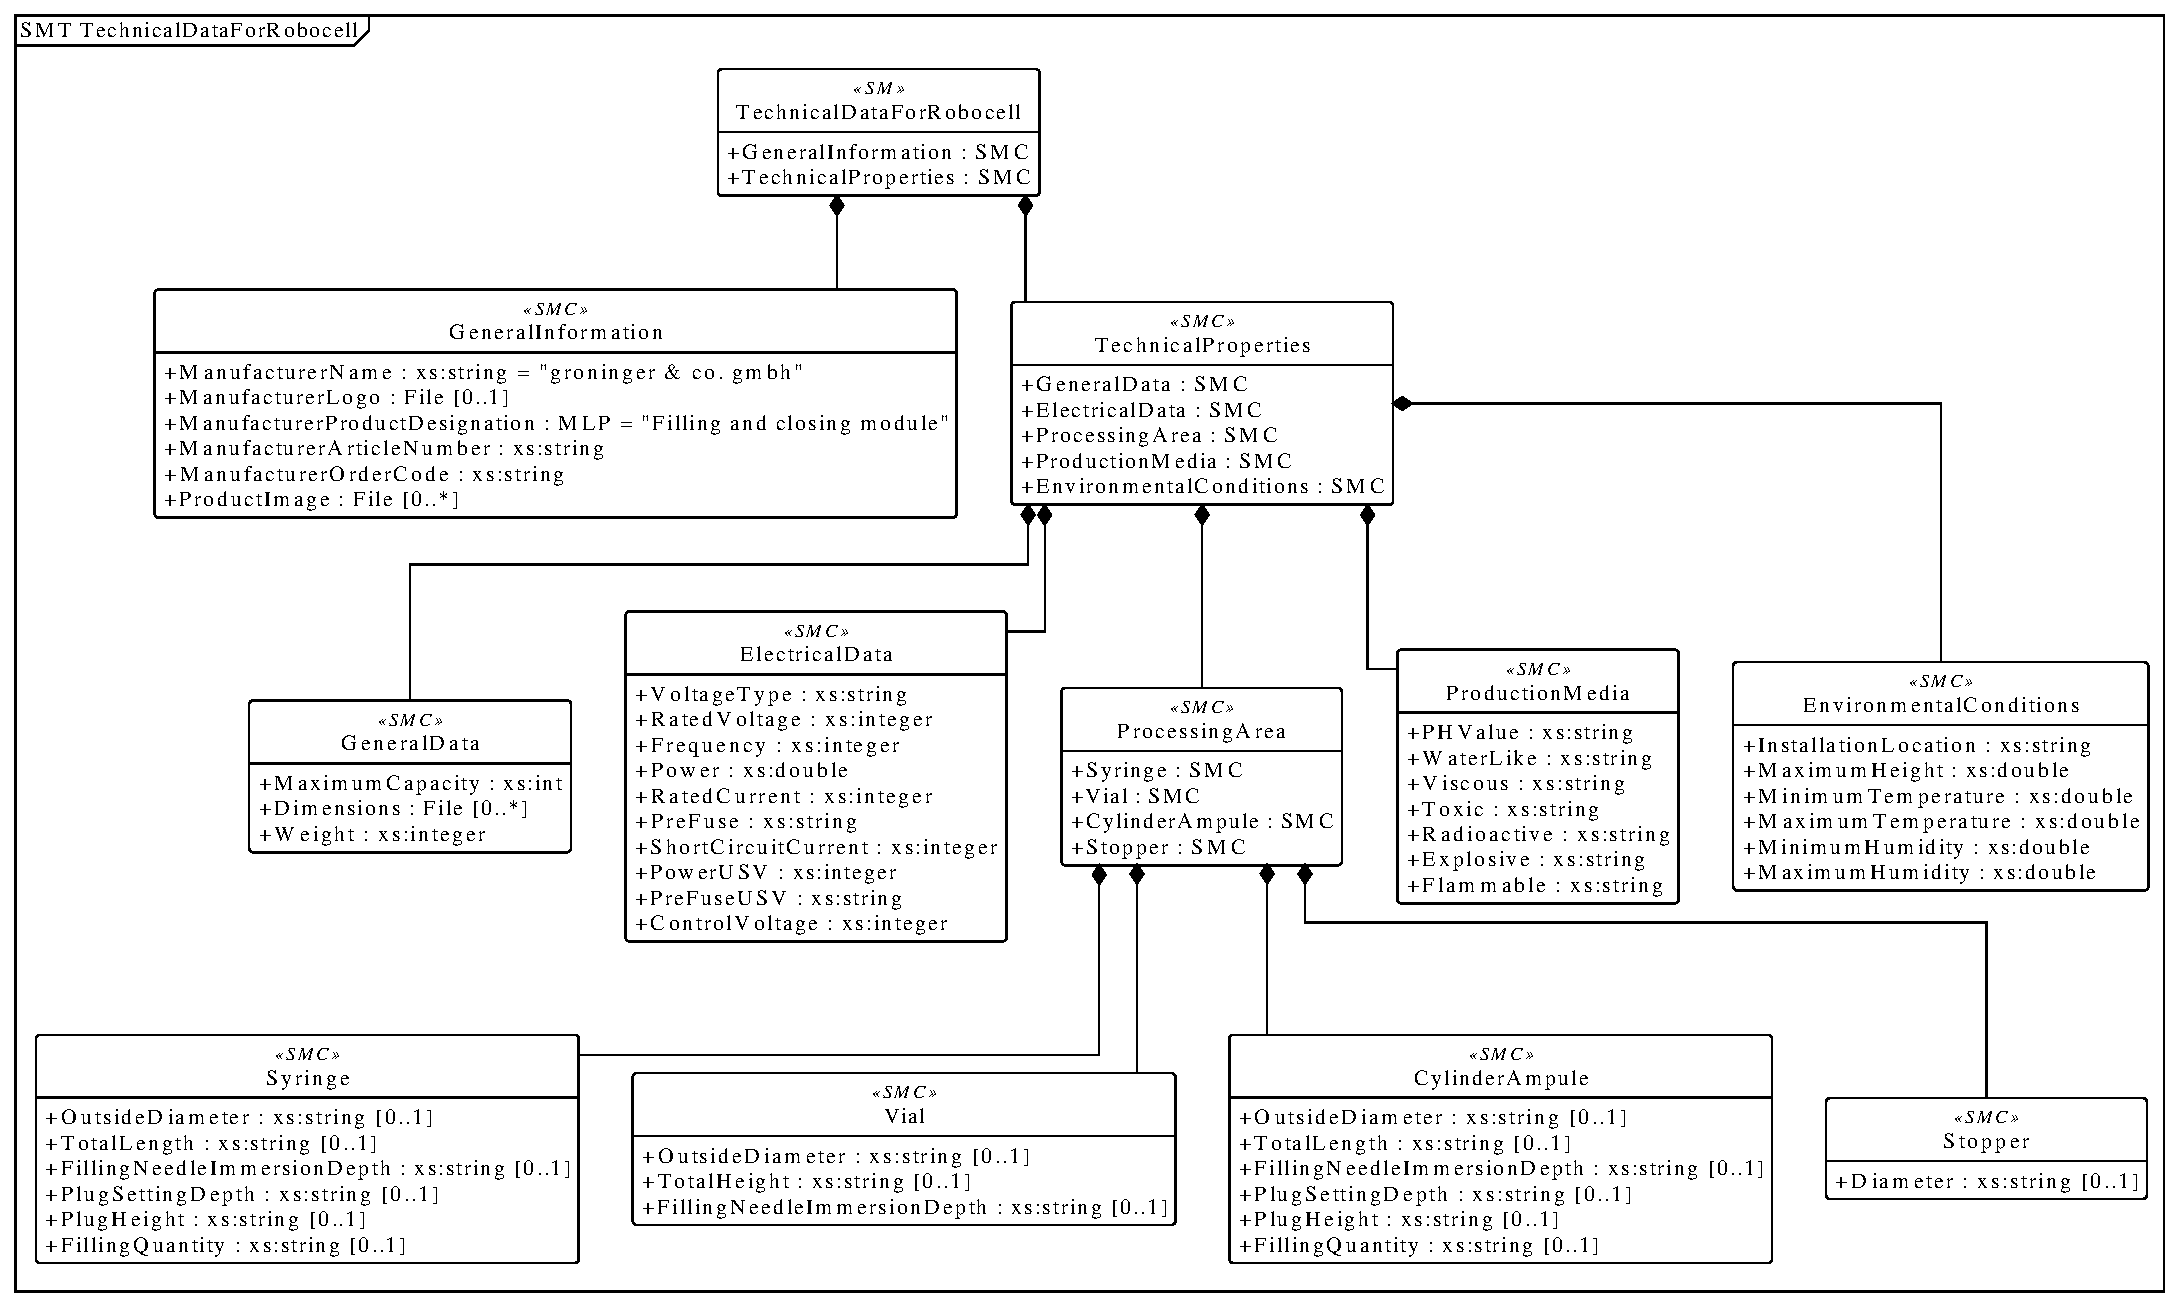
\includegraphics[width=1\textwidth]{Bilder/UML/tehcnicalDataForRobocell.pdf}
%     \caption{!!!}
%     \label{fig:!!!}
% \end{figure}

\subsubsection{Automatisiertes Befüllen mit strukturierten Daten}
Nach der Erstellung eines Typ-Submodells stellt sich die Frage, wie dieses effizient mit konkreten Informationen befüllt und anschließend in eine vollständige \acs{aas}-Instanz eingebettet werden kann.
In der Praxis liegen die hierfür benötigten Daten häufig bereits strukturiert in bestehenden Unternehmenssystemen vor, beispielsweise in \acs{plm}- oder \acs{erp}-Systemen.

Da eine direkte Anbindung solcher Systeme im Rahmen dieser Arbeit nicht möglich ist, wird das automatisierte Befüllen exemplarisch anhand vorgegebener Beispieldaten umgesetzt.
Diese enthalten technische Informationen, wie sie typischerweise in den Unternehmenssystemen vorliegen, und bilden die Grundlage für die automatisierte Erstellung des Instanz-Submodells Technische Daten.

Für die technische Umsetzung bietet sich ein Skript an, das diese Daten automatisiert in die vorgegebene Submodellstruktur überträgt und anschließend in Form einer Typ-2-\acs{aas} bereitstellt.
In diesem Projekt wird dazu die serverseitige JavaScript-Laufzeitumgebung Node.js \cite{nodejs} verwendet, da sie eine einfache Verarbeitung von JSON-Daten sowie eine unkomplizierte Kommunikation mit REST-Schnittstellen ermöglicht. 
Als Basis werden drei zentrale Komponenten benötigt:

\begin{enumerate}[noitemsep, leftmargin=*, label=\textbf{\arabic*.}]
    \item \textbf{Datenquelle:} Technische Produktinformationen
    \item \textbf{Submodell-Vorlage:} Struktur und Semantik des Submodells
    \item \textbf{AAS-Vorlage:} Aufbau und Struktur der \acs{aas}-Instanz
\end{enumerate}

Die Datenquelle liegt im JSON-Format vor und ist hierarchisch aufgebaut.
Sie besteht aus mehreren verschachtelten Schlüssel-Wert-Paaren.
Jeder Schlüssel dient als eindeutiger Bezeichner und entspricht einem idShort-Wert eines Submodellelements innerhalb der Submodell-Vorlage.
Diese Vorlage ist so konzipiert, dass an den relevanten Stellen Platzhalter vorhanden sind, die während der Ausführung des Skripts mit den zugehörigen Werten aus der Datenquelle befüllt werden können.

Nach dem Befüllen des Submodells mit konkreten Werten muss dieses in eine zugehörige \acs{aas}-Instanz eingebunden werden. 
Die AAS-Vorlage definiert hierfür die grundlegende Struktur der \acs{aas} in einer separaten JSON-Datei. 
Diese enthält jedoch noch keine spezifischen Identifikatoren, wie beispielsweise die eindeutige ID der \acs{aas} oder des zugehörigen Assets. 
Um diese hinzuzufügen, können während der Skriptausführung zufällige UUIDv4-Werte generiert und an den entsprechenden Stellen in die Vorlage eingefügt werden.

Im Anschluss daran gilt es, die \acs{aas} in einer Industrie-4.0-Anwendung bereitzustellen. 
Hierfür kann erneut Eclipse BaSyx genutzt werden, wobei die AAS sowie das zugehörige Submodell, analog zur Möglichkeit~c) (REST-API) aus Kapitel~\ref{sec:bereitstellungAAS}, eingebunden werden kann.

% \subsubsection{Potenziale des KI-Einsatzes}

\subsection{Anwendungsfall KI in der Industrie 4.0}

\subsubsection{Anomaliererkennung mit maschinellem Lernen}
Datenquelle
Umsetzung mit pytorch
Modelltraining mit Autoencoder
Modell sepcihern mit onnx


Bild erst in Ergebnissse

\subsubsection{Modellverwaltung mit der \acs{aas}}

